\section{Analog Signal Chain}
\begin{minipage}{11cm}
	Embeddes Systems interact with the the Outer Real World. In this Environment, many Signals in the outer Real World are Analog. Analog Signals must be transferred into their Digital Representation to be processed. 
\end{minipage}
\begin{minipage}{6cm}
	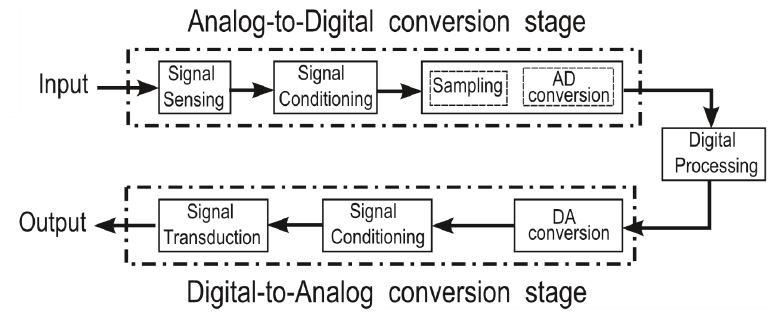
\includegraphics[width=8cm]{images/signalchain.jpg}
\end{minipage}
%TODO Add some picture of electronic ciruits...??
\subsection{Mixed-Signal Processing Chain}
\begin{itemize}
	\item Signal Chain
	\subitem refers to a series of Signal-Conditioning Electronic Components connected to each other
	\item Signal Sensing
	\subitem Active and Passive Sensors, Sensor Characteristics
	\item Signal Conditioning
	\subitem Amplification,Linearizing, Filtering
	\item Signal Transduction
	\subitem Active and Passive Sensors, Sensor Characteristics
\end{itemize}
\subsection{Comparator, ADC, DAC}
\clearpage
\pagebreak